\documentclass{article}

\usepackage{amsmath}
\usepackage{listings}
\usepackage{graphicx}

\title{Homework 2}

\author{Crist\'obal Armaza, Chris Silvia}

\begin{document}

\maketitle

\section*{Organization}

We met and derived the formulas for P1 and P2. Christopher wrote the solution to these problems.
We then started a new Github repo to write and co-edit the code for the finite differene coefficients
as well as the tests to compute the error. Crist\'obal wrote the solution to P3 and Christopher
wrote the solution to P5.

\section{Lagrange Interpolating Polynomial}

We are trying to write a polynomial which, if we are considering
	the points $x_0, \dots, x_n$, is equal to one at $x_i$,
	and equal to zero for all $x_j$, with $j \neq i$.
We exhibit this polynomial below.

\begin{align}
f_i(x) & = \prod_{j \neq i} \frac{x - x_j}{x_i - x_j}
\end{align}

Note that $f_i(x_i) = \prod_{j \neq i} \frac{x_i - x_j}{x_i - x_j}$,
	and since all of the numerators and denominators are equal,
	we can see that $f_i(x_i) = 1$.
For $f_i(x_k) = \prod_{j \neq i} \frac{x_k - x_j}{x_i - x_j}$,
	if $k \neq i$, since $j$ ranges over all indices except $i$,
	one of the $j$'s will be equal to $k$.
That will make the numerator zero, and thus the whole product
	will be zero.
Therefore, $f_i(x_k) = \delta_{ik}$.

If we want our polynomial to have the value $y_i$ at each
	point $x_i$, we can sum several of these polynomials, so that
	the resultant polynomial has the characteristics which we desire:

\begin{align}
f(x) & = \sum_i y_i f_i(x) \\
& = \sum_i y_i 
	\left( \prod_{j \neq i} \frac{x-x_j}{x_i-x_j} \right)
\end{align}

This polynomial has the required values at each point.

\section{Differentiating a Lagrange Interpolating Polynomial}

Given the definition of $f_i(x)$ given above, we can compute
	the derivative of $f_i(x)$ with respect to $x$.

\begin{align}
\frac{d f_i(x)}{dx} & = \sum_{\begin{matrix}k=0\\k\neq i\end{matrix}}^n 
	\frac{1}{x_i - x_k}
	\left( \prod_{
		\begin{matrix} j = 0 \\ j \neq k\\j \neq i \end{matrix}}^{j=n}
		\frac{x - x_j}{x_i - x_j} \right)
\end{align}

Therefore, for the whole approximating function $f(x)$, we have:

\begin{align}
\frac{df}{dx}(x) & = \sum_{\begin{matrix}i=0\end{matrix}}^n
	y_i
	\sum_{\begin{matrix}k=0\\k\neq i\end{matrix}}^n
	\frac{1}{x_i - x_k}
	\left( \prod_{
		\begin{matrix} j = 0 \\ j \neq k\\j \neq i \end{matrix}}^{j=n}
		\frac{x - x_j}{x_i - x_j} \right)
\end{align}

This can be interpeted as a dot product.
If we consider the vector $\vec{D}(x)$ given by:

\begin{align}
D_i(x_l) & = 
	\sum_{\begin{matrix}k=0\\k\neq i\end{matrix}}^n
	\frac{1}{x_i - x_k}
	\left( \prod_{
		\begin{matrix} j = 0 \\ j \neq k\\j \neq i \end{matrix}}^{j=n}
		\frac{x - x_j}{x_i - x_j} \right)
\end{align}

Then if we consider the vector $\vec{y} = \{ y_0, \dots, y_n \}$,
	then $\frac{df}{dx}(x) = \vec{D}(x) \cdot \vec{y}$.

\subsection{Computing the Derivative at the Stencil Points $x_0, \dots x_n$}
  
Suppose $x = x_l$ is one of the coordinates.
Then, $D_i(x_l)$ is given by:

\begin{align}
D_i(x_l) & = 
	\sum_{\begin{matrix}k=0\\k\neq i\end{matrix}}^n
	\frac{1}{x_i - x_k}
	\left( \prod_{
		\begin{matrix} j = 0 \\ j \neq k\\j \neq i \end{matrix}}^{j=n}
		\frac{x_l - x_j}{x_i - x_j} \right)
\end{align}

However, this can be greatly simplified.
If $x_l = x_i$, then we see that the product terms all drop out,
	since the numerators and denomiators are all equal.
If $x_l \neq x_i$, then the product would only be nonzero for the
	case where $k=l$.
Therefore, only that term in the sum survives.
We show the special cases for $D_i(x_l)$ below:

\begin{align}
D_i(x_i) & = \sum_{\begin{matrix}k=0\\k\neq i\end{matrix}} \frac{1}{x_i - x_k}\\
\begin{matrix}D_i(x_l)\\l \neq i\end{matrix} & = \frac{1}{x_i - x_l} 
	\prod_{
		\begin{matrix} j = 0 \\ j \neq l\\j \neq i \end{matrix}}^{j=n}
		\frac{x_l - x_j}{x_i - x_j} 
\end{align}

\section{Finite Difference Scheme Code}

The code snippet below implements a stencil to compute the derivative
	at an arbitrary point $x$.

\lstset{language=C++}
\begin{lstlisting}
/*  FUNCTION: 1st derivative of f(x).
    Given a stencil, it generates the finite diff coefficients

    x = point at which dfdx is evaluated
    ns = number of points on the stencil
    xs = array of locations of stencil points
    D = array to save coefficients
*/
void dfdx(double x, int ns, double *xs, double *D){
    // For the k-th stencil point, calculate its 
    //     coefficient and store it in D[k].
    double aux;
    for(int i=0; i<ns; i++){
        D[i] = 0;
        for(int k=0; k<ns; k++){
            aux = 1/(xs[i]-xs[k]);
            for(int j=0; j<ns; m++){
                if(j!=i && j!=k)
                    aux *= (x - xs[j])/(xs[i] - xs[j]);
            }
            D[k] += aux;
        }
    }
}
\end{lstlisting}

\section{Formal Accuracy of Finite Difference Scheme}

Given an $n$-point stencil, which is a series of points 
	$x_0, \dots, x_n$, 
	and a point at which the derivative is to be computed,
	$x$, we compute coefficients which can be used to compute
	the derivative at $x$ based on the values of the function
	$f$ at the points $x_0, \dots, x_n$.

This is done by deriving an expression to find a polynomial
	which interpolates all $n$ points, assuming that we know
	the value of $f$ at each point..
This polynomial is thus of order $n-1$.
The polynomial is derived from a taylor series, which 
	necessarily contains factors of the separation between
	points, $dx$.

The derivative of the interpolating polynomial is of order
	$n-2$.
If we consider the polynomial of infinite order which perfectly
	matches $f'$, given that we have a polynomial approximation
	of order $n-2$, and assuming that the successively
	higher powers of $dx$ make the lowest order polynomial
	term dominant, the difference between $f'$ and the interpolating
	derivative polynomial of order $n-2$ is a polynomial of 
	order $n-1$.
In summary, our approximated derivative matches all the polynomial
	coefficients up to $n-2$, leaving $n-1$ the largest
	contribution to the error.

Since the polynomial of order $n-1$ comes with factors of 
	the separation $dx$, the error \emph{at each point}
	is proportional to $dx^{n-1}$.

For example, with a 5th order method, the expected error 
	at each point should decrease 4 db/dec.


\section{Computation of mesh}

In this section, we consider a mesh in which the point $x_i$, 
	$i$ ranging from $0$ to $n$, the points are distributed as:

\begin{align}
x_i & = \frac{i}{n} + \frac{1}{10} \sin \left( \frac{2 \pi i}{n} \right)
\end{align}

We are using our finite-difference scheme code to generate a five-point
	computational stencil.
This stencil varies spatially, as the point distribution changes.

Using the function $f(x) = \tanh ( 10 x - 5 )$, we compare the analytical
	derivative with the numerical derivative.
The code which produced this figure is given in Appendix A.

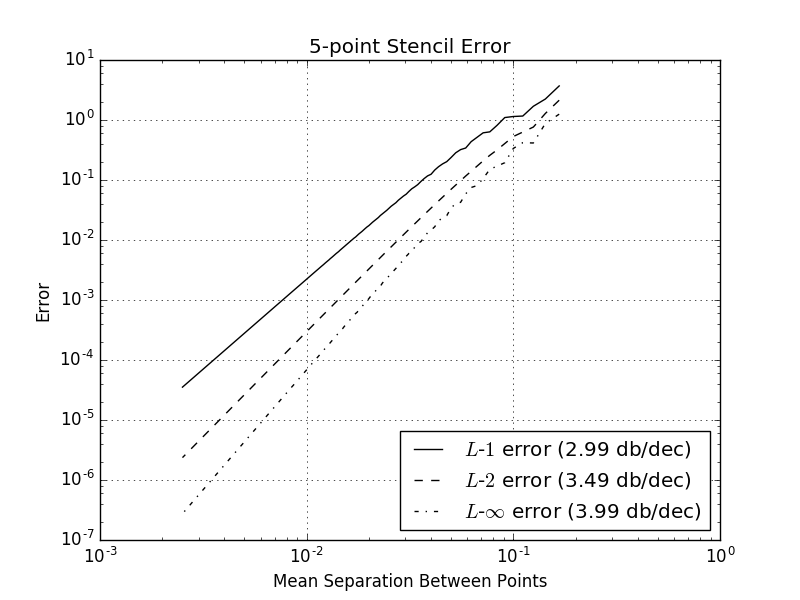
\includegraphics[width=\textwidth]{ErrorDecrease.png}

For some reason, the $L$-$1$ error has a slope of 3,
	the $L$-$2$ error has a slope of 3.5,
	and the $L$-$\infty$ error has a slope of 4.
This result surprised us, and we aren't quite sure why the errors
	decrease in this way.

If every individual point's error is decreased in the 4th order
	of the mean point separation, then this accounts for the
	$L$-$\infty$ error's slope.

If every individual point's error is decreased by the 4th power
	of the mean separation, but there are more points as the inverse
	1st power of the mean separation, then the total $L$-$1$ error
	may decrease as the third power of the separation, as the product
	of these two.

I am still unsure why the $L$-$2$ error decreased by the 3.5th
	power of the mean separation.

\subsection{Boundaries of the Mesh}

The computation above was performed only on the interior points,
	with at least two neighbors.
We referred earlier to the $D$ matrix, where $D_{ij} = D_i(x_j)$.
This was done by computing the full $D$ matrix for a 5-point stencil,
	and then selecting the row corresponding to the center point.
In order to compute the derivatives on the boundary, one need only select
	the row corresponding to the boundary point.
This is a 4th order method throughout the simulation region.

However, this is not necessarily what we might want.
If we want to preserve the pentadiagonal structure, the first row
	and last row can only contain three nonzero entries.
Similarly, the second and second-to-last rows can only contain four
	nonzero entries.
The solution is to make a $D$ matrix for the first three (or four)
	points, and then select the row corresponding to the relevant point.
While this preserves the diagonal structure of the matrix, this is not
	a  4th order matrix all throughout the simulation region.

The final way to compute the boundaries is if we perscribe the values 
	of the function past the boundary of the simulation region,
	or if we perscribe the value of the function and the derivative
	at the boundary, we can preserve the 5th order character
	of the method, as well as the pentadiagonal structure.

\appendix
\section{Code Appendix}
\lstset{language=python}
\lstinputlisting{make_err.py}

\end{document}
